\section{Osnovni problem}\label{sec:1}

Analiziramo optimalno vožnjo avtomobila z začetno hitrostjo $v_0$ do semaforja na razdalji $L$, ako vemo, da se rdeča luč spremeni v zeleno čez $t_0$. Pri tem ne želimo zapeljati v rdečo luč, zato definiramo pogoj za razdaljo $\int_0^{t_0} v(t) \, dt = L$, velja za tudi začetni pogoj $v(0) = v_0$. Najbolj optimalno (udobno in varčno) vožnjo pa opišemo kot vožnjo s čimmanj pospeški in pojemki $\int_0^{t_0} \dot{v}^2(t) \, dt = \text{MIN}$. Problem zapisan kot funkcional z Lagrangeevo funkcijo se glasi: 
$$\alpha(\dot{v}, v) = \vec{v}^2 - \lambda \, v \text{, } \quad F = \int_0^{t_0} \alpha \, dt \text{,}$$
kjer je $\lambda$ neznani multiplikator. Ker iščemo ekstrem (minimum) funkcionala, lahko rešitev pridobimo iz Euler-Lagrangeevih enačb $\frac{d}{dt} \left( \frac{\partial \alpha}{\partial \dot{v}} \right) - \frac{\partial \alpha}{\partial v} = 0$. Tako dobimo zvezo $ 2 \, \ddot{v} + \lambda =0$, iz tega splošno rešitev enačbe $v(t) = - \frac{\lambda}{4} \, t^2 + A \, t + B$ in z upoštevanjem začetnega pogoja in pogoja za razdaljo dobimo iskano rešitev
$$v(t) = - \frac{3}{2 \, t_0^3} \, (L - v_0 \, t_0) \, t^2 + A \, t + v_0 \text{.}$$

Neznanko $A$ določimo s pomočjo dodatnega robnega pogoja. Lahko izberemo, da je hitrost poljubna, vendar mora biti pri semaforju ekstremna $\dot{v}(t_0) = 0$ ali enaka največji dovoljeni hitrosti pri semaforju $v(t_0) = v_{\text{max}}$ in tako dobimo vrednost $A$ ter sledeča izraza za potek hitrosti za oba primera robnega pogoja:
$$v(t) = \frac{3 \, (L- v_0\, t_0)}{2 \, t_0^3} \, (2 \, t_0 \, t - t^2) + v_0 \text{ in }$$
$$v(t) = \frac{3 \, (2\, L - v_0\, t_0 - v_{\text{max}}\, t_0)}{t_0^3} \, (t_0 \, t - t^2) + \frac{ v_{\text{max}} - v_0}{t_0} \, t+ v_0 \text{.}$$

Zgoraj omenjeno rešitev problema ($2 \, \ddot{v} + \lambda =0$) prepišemo v v brezdimenzijsko obliko z uvedbo $\Tilde{v}= \frac{v}{V} \text{ in } \Tilde{t}= \frac{t}{T} \text{,}$ kjer sta $V$ in $T$ referenčni konstanti. Po izračunu dvojnega odvoda hitrosti
$$\frac{d^2v}{dt^2} = \frac{d}{dt} \left( \frac{V}{T} \, \frac{d\Tilde{v}}{d\Tilde{t}} \right) = \frac{V}{T^2} \, \frac{d^2\Tilde{v}}{d\Tilde{t}^2}$$
lahko zapišemo enačbo problema v brezdimenzijski obliki, kjer smo pridobili dodatno brezdimenzijsko konstanto $\Pi = \frac{\lambda \, T^2}{2 \, V}$
$$\ddot{\Tilde{v}} + \Pi = 0 \text{.}$$

Predpostavimo, da se peljemo s hitrostjo 90 km/h in naletimo na semafor čez 300 m z rdečo lučjo. Slika \ref{fig:90_do_50} prikazuje, kako vpliva zahtevani čas prevožene razdalje na potek hitrosti za oba primera, opisana zgoraj. Opazimo, da lahko pri pogoju ekstremne hitrosti močno presegamo največjo dovoljeno hitrost pri semaforju, vendar tudi pri pogoju z $v_{\text{max}} = 50$ km/h
lahko pri zelo kratkem času (npr. $t_0 = 10$ s) v bližini semaforja močno presegamo omejitev. Rešitev za 15 s pri upoštevanju maksimalne hitrosti je skoraj linearna, kar je posledica naključnega ujemanja podatkov. Tudi razlika med rešitvama za oba dodatna pogoja je tukaj najmanjša, dočim se najbolj razlikujeta pri krajših časih $t_0$.

\begin{figure}[ht!]
    \centering
    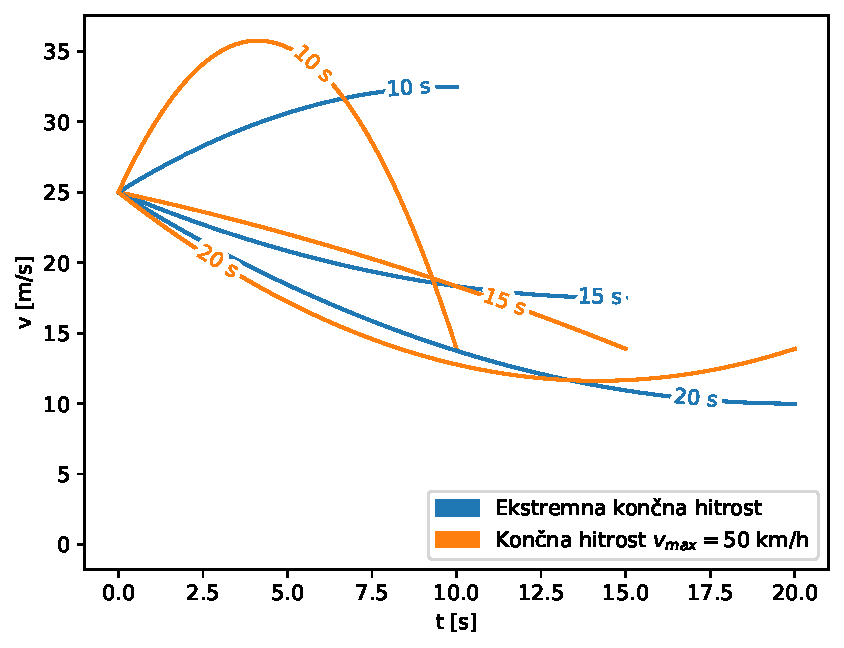
\includegraphics[width=0.72 \textwidth]{1.nal_slike/90_do_50kmh.pdf}
    \caption{Poteh hitrosti od začetne $v_0 = 90$ km/h do semaforja čez $L = 300$ m za različne čase $t_0$ do zelene luči. Pri tem je omejitev pri semaforju $v_{\text{max}} = 50$ km/h.}
    \label{fig:90_do_50}
\end{figure}

Na sliki \ref{fig:0_do_50} je prikazan potek hitrosti med dvema semaforjema, kjer odpeljemo s prvega takoj po prižigu zelene luči in želimo pripeljati skozi drugega natanko ob prižigu zelene luči in ne želimo prekoračiti omejitve hitrosti. Opazimo, da nam variacijski račun upošteva le omejitev hitrosti pri času $t_0$, kar je definirano pri robnem pogoju, hitrost pa lahko preseže omejitev na vmesnem delu, saj rešujemo integralsko enačbo, kjer mora biti prevožena razdalja enaka razdalji $L$ do semaforja. Za upoštevanje omejitve tekom celotnega potovalnega časa, bi potrebovali drugačen fizikalni model.

\begin{figure}[H]
    \centering
    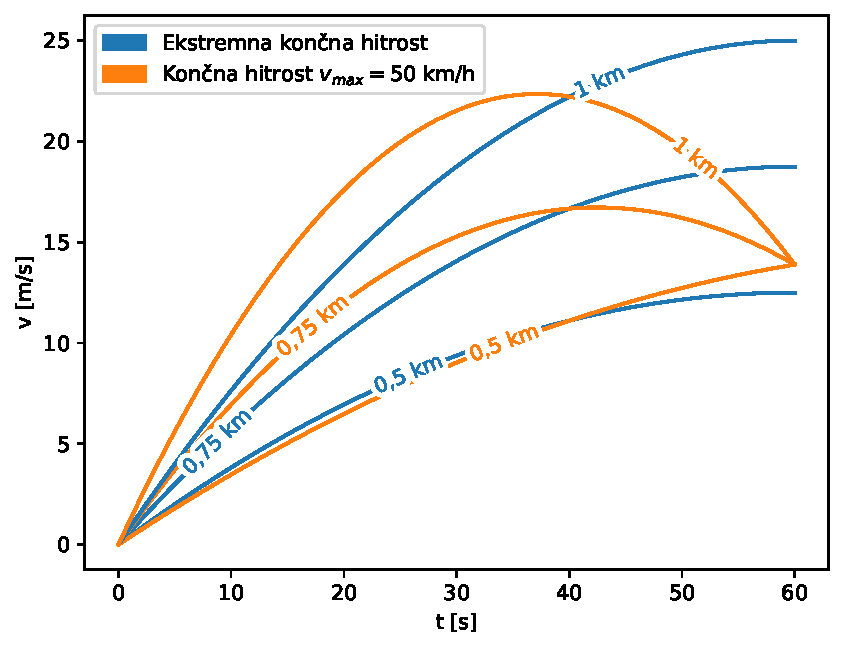
\includegraphics[width=0.72 \textwidth]{1.nal_slike/0_do_50kmh.pdf}
    \caption{Poteh hitrosti od začetne $v_0 = 0$ km/h do med semaforjema z intervalom  $t_0 = 60$ s za različne razdalje $L$ med njima. Pri tem je omejitev hitrosti $v_{\text{max}} = 50$ km/h.}
    \label{fig:0_do_50}
\end{figure}

Iz primerov je moč sklepati, da začetna in končna hitrost spreminjata lego parabole, razdalja in čas pa določata njeno ukrivljenost, saj imamo pogoj, da mora biti prevožena razdalja enaka razdalji do semaforja, kar je razvidno iz Slike \ref{fig:0_do_50}.

\section{Višje potence v funkcionalu}

Spremenimo potenco v $p$ v Lagrangeevi funkciji, zato se spremeni tudi fukcional, ki ga obravnavamo $F = \int_0^{t_0} \left[ \dot{v}^{p}(t) - \lambda \, v(t) \right] \, dt$, tako dobimo novo splošno rešitev:
$$v(t) = - \frac{p -1}{\lambda} \, \left( C_1 - \frac{\lambda \, t}{p} \right)^{\frac{p}{p-1}} + C_2 \text{.}$$
Ob upoštevanju robnega in začetnega pogoja ter pogoja za razdaljo pridobimo vrednosti konstant $C_1$, $C_2$ in $\lambda$. Tako dobljen predpis hitrosti ima poleg prejšnjih treh prostih parametrov še novega – potenco $p$. Ker je tak izraz preveč kompleksen za splošen analitičen izračun, smo izvedeli izračun predpisa hitrosti s številčnimi vrednostmi za vsako potenco $p$ posebej.

\subsection{Sode potence}

Potence so sode, ko $p = 2, 4, 6 ...$. Iz slike \ref{fig:sode_potence} je razvidno, da se z višanjem potence graf hitrosti približuje linearni funkciji.

\begin{figure}[ht!]
    \centering
    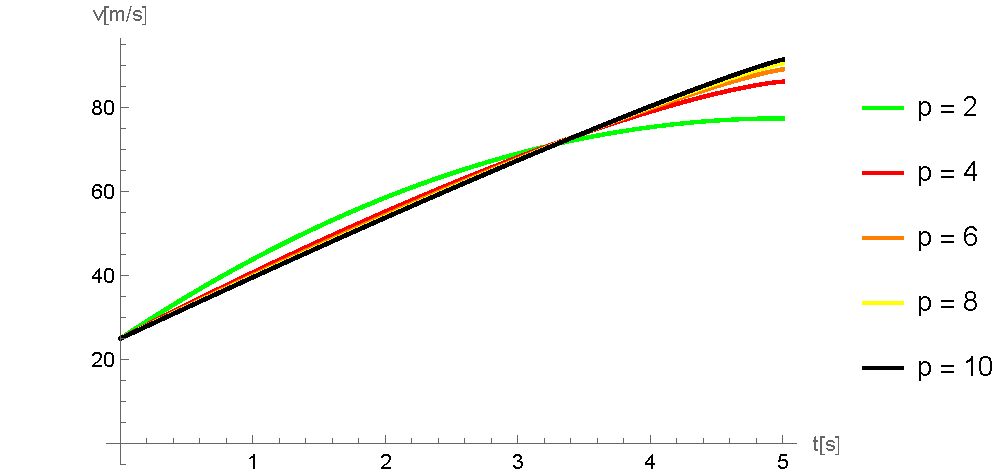
\includegraphics[width=0.8 \textwidth]{1.nal_slike/sode_potence.pdf}
    \caption{Sode potence $p$ pospeška v funkcionalu pri prostih \linebreak parametrih $t_0=5$ s,  $v_0=90$ km/h in $L=300$ m.}
    \label{fig:sode_potence}
\end{figure}

V limitnem primeru, ko $p \to \infty$ bi tako imeli enakomerno pospešeno gibanje s predpisom hitrosti $v(t) = a \, t + v_0$.

Pri $p=2$ je ugotovljeno ujemanje z rešitvijo iz prejšnjega poglavja, pri enakih preostalih prostih parametrih problema.

\subsection{Lihe potence}

Potence so lihe, ko $p = 3,5,7 ...$, iz tehničnih razlogov je potenca $p=1$ izpuščena, saj tak primer povzroči ulomek $\frac{p}{p-1}$ z ničlo v imenovalcu. Na sliki \ref{fig:lihe_potence} so prikazane lihe potence, in iz primerjave z rezultati s sodimi na sliki \ref{fig:sode_potence} lahko opazimo, da izkazujejo enak trend približevanja enakomerno pospešenemu gibanju z zviševanjem potenc.

\begin{figure}[H]
    \centering
    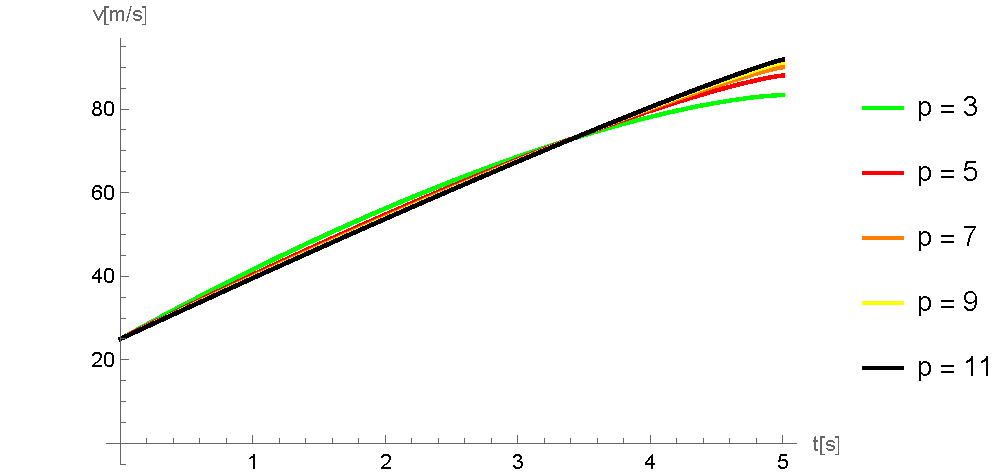
\includegraphics[width=0.8 \textwidth]{1.nal_slike/lihe_potence.pdf}
    \caption{Lihe potence $p$ v funkcionalu pri preostalih \linebreak prostih parametrih enakih kot na sliki \ref{fig:sode_potence}.}
    \label{fig:lihe_potence}
\end{figure}
\section{Kvadratični člen hitrosti v funkcionalu}

V tem primeru definiramo Lagrangeevo funkcijo z dodatnim členom hitrosti \linebreak $\alpha(\dot{v}, v) = \vec{v}^2 + C \, v^2 - \lambda \, v$, ki nastopa v funkcionalu $F = \int_0^{t_0} \alpha \, dt$. V tem primeru bomo z reševanjem funkcionala pridobili diferencialno enačbo, ki bo poleg neznane $\lambda$ vsebovala tudi neznanko $C$, ki predstavlja nov prosti parameter. Tako dobljena Euler-Lagrangeeva enačba, ki jo rešujemo 
$$2 \, \ddot{v}(t) - 2 \, C_0 \, v(t) + \lambda = 0$$
ima prekompleksno analitično rešitev, katere ni smiselno pisati v poročilo. Zaradi numeričnih razlogov, izračun za $C_0 = 0$ ni bil mogoč, zato je bil izveden za sicer neničelno vrednost, a zelo blizu ničelne.

\begin{figure}[ht!]
    \centering
    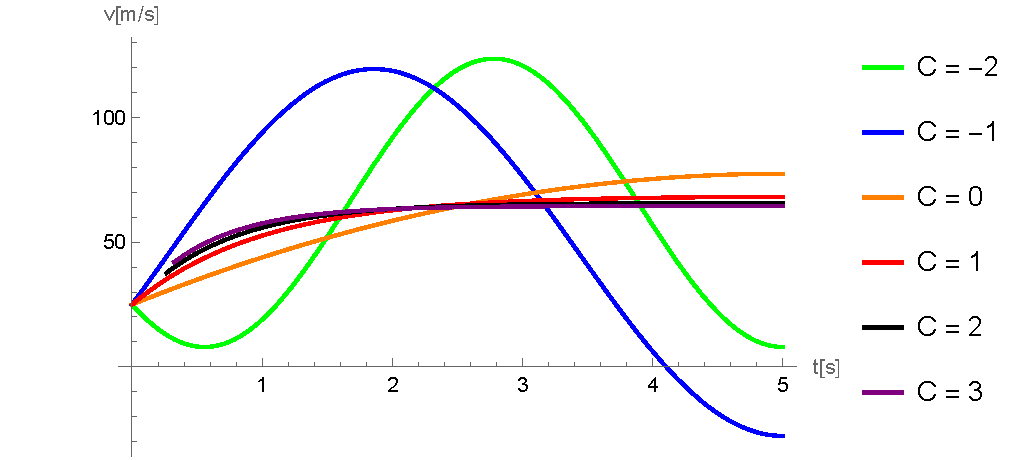
\includegraphics[width= 0.85 \textwidth]{1.nal_slike/clen_hitrosti.pdf}
    \caption{Vpliv parametra $C_0$ (na sliki označen kot $C$) na potek hitrosti pri \linebreak preostalih prostih parametrih enakih kot na slikama \ref{fig:sode_potence} in \ref{fig:lihe_potence}.}
    \label{fig:vpliv_C0}
\end{figure}

Opazimo, da povečevanje pomembnosti pogoja za minimizacijo hitrosti vse bolj teži k enakomernem gibanju, saj je v funkcionalu vedno bolj ‘kaznovana’ prevelika hitrost. medtem ko primera za negativni parameter $C_0$ izkazujeta, da le-to vzpodbuja čim večje hitrosti, kar se odraža v nihanju, ki se z zmanjševanjem parametra le stopnjuje. V primeru ko $C_0 = -1$ pride tudi do negativne hitrosti, kar je za vozilo na cesti nerealno in celo potencialno nevarno.

Ob dodatnem razmisleku lahko domnevamo, da bi parameter $C_0$ predstavljal konstanto pri kvadratičnem zakonu zračnega upora ($F_u = k \, v^2$), saj ima avtomobil dolžine 4 m Reynoldsovo število reda velikosti $10^6$ pri hitrostih nad 15 km/h, kar je močno v turbulentnem področju. Za primer avtomobila Volvo 480 bi ta konstanta znašala $k = 0,44$ kg/m in glede na porabo goriva optimalen potek hitrosti bi bil tako za vsako vozilo specifična krivulja, kjer zaradi fizikalnega pomena konstante nikoli ne pride do tako ekstremnih primerov nihanja hitrosti, kot je prikazano na sliki \ref{fig:vpliv_C0}.

\section{Periodične rešitve}

Ob upoštevanju, da je hitrost pri semaforju, do katerega peljemo ekstremna (pospešek je enak 0), dobimo iz rešitve funkcionala sledečo enačbo, kot je že opisano v poglavju \ref{sec:1}
$$v_i(t) = \frac{3 \, (L- v_0\, t_0)}{2 \, t_0^3} \, (2 \, t_0 \, t - t^2) + v_0$$
kjer optimiziramo potek hitrosti na vsakem intervalu med semaforji posebej, zato ob vsakem prevoženem semaforju upoštevamo, da se hitrost iz prejšnjega intervala ohranja. Ako imajo semaforji enake intervale $t_0$, je definicija trivialna
$$v_i = v_{i-1}(i \cdot t0) \text{.}$$

Na tak način pridobljene rešitve po intervalih lahko ‘zlepimo’ v enoten graf, prikazan na sliki \ref{fig:periodično_nezvezno}. Dobljen rezultat ima sicer ujemajoče se vrednosti hitrosti na prehodu semaforja, vendar, kot je razvidno na grafu pospeškov, le-to ni ujemajoče, zato je tudi potek hitrosti nezvezen. Potrebno bi bilo upoštevati, da se poleg hitrosti pri prehodu semaforja skladajo tudi pospeški.

\begin{figure}[H]
    \centering
    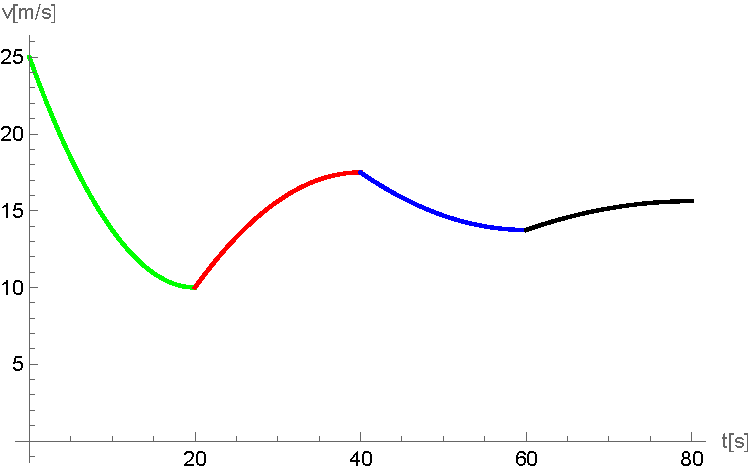
\includegraphics[width=0.7 \textwidth]{1.nal_slike/hitrost_periodično.pdf}
    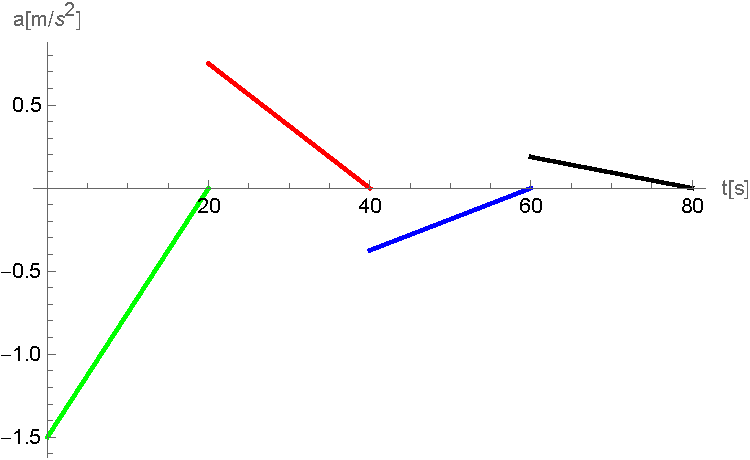
\includegraphics[width=0.7 \textwidth]{1.nal_slike/pospešek_periodično.pdf}
    \caption{Potek hitrosti in pospeška pri rešitvi za 4 semaforje na razdaljah $L=300$ m in intervalih $t_0 = 20$ s ter začetne hitrosti $v_0 = 90$ km/h ob upoštevanju enake hitrosti ob prehodu semaforja.}
    \label{fig:periodično_nezvezno}
\end{figure}

Ako pa upoštevamo, da je pospešek na začetku intervala $a(0)=a_0$, dobimo sledeč izraz za potek hitrosti
$$v_i(t) =  a_0 \, t +  v_0 + \frac{2\, L - a_0\, t_0^2 - 2\, t_0\, v_0}{2\, t_0^3}\, 3\, t^2 \text{.}$$
Sedaj lahko definiramo tudi enak pospešek pri prehodu semaforja za primer enakomernih intervalov semaforjev
$$a_i = \dot{v}_i= \dot{v}_{i-1}(i \cdot t0) \text{.}$$

Kot je prikazano na sliki \ref{fig:periodično_zvezno} je tokrat potek hitrosti zvezen, potek pospeškov pa ne. Sicer pa je taka nezveznost pospeška mogoča ob nagli spremembi stopalke za plin. Razlikuje se tudi od poteka na sliki \ref{fig:periodično_nezvezno}, čeprav so razdalje in intervali med semaforji enake, saj smo morali prilagoditi novo uvedeni parameter začetnega pospeška $a_0$, ki je bil umerjen ročno, tako, da je rešitev kar najbolj smiselna. V tem primeru znašata -1,732 051 0 in \linebreak -1,732 050 5 m/s$^2$, kar ustreza krivuljama na spodnjem grafu z najmanj ‘podivjanima’ potekoma hitrosti in pospeška. Opazimo, da je hitrost pri bližnjih semaforjih stabilna, začetni pospešek pa predvsem vpliva na hitrost daleč od izhodišča, zato je za več semaforjev potrebni bolj strogi začetni pogoji, če želimo prevoziti vsa križišča optimalno.

\begin{figure}[H]
    \centering
    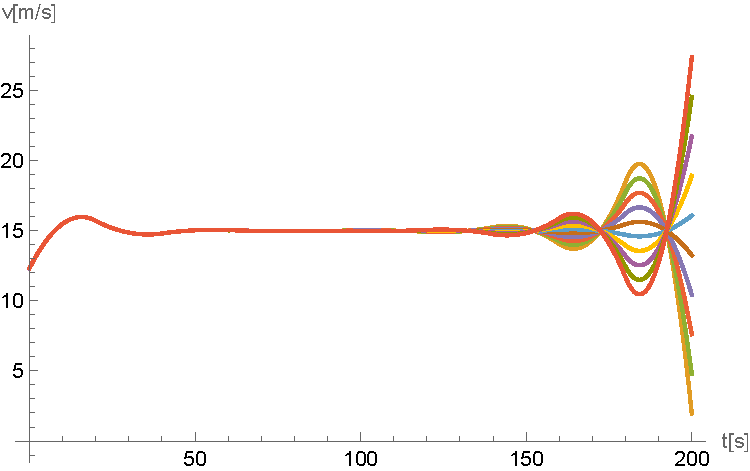
\includegraphics[width=0.7 \textwidth]{1.nal_slike/hitrost_periodično_zvezno.pdf}
    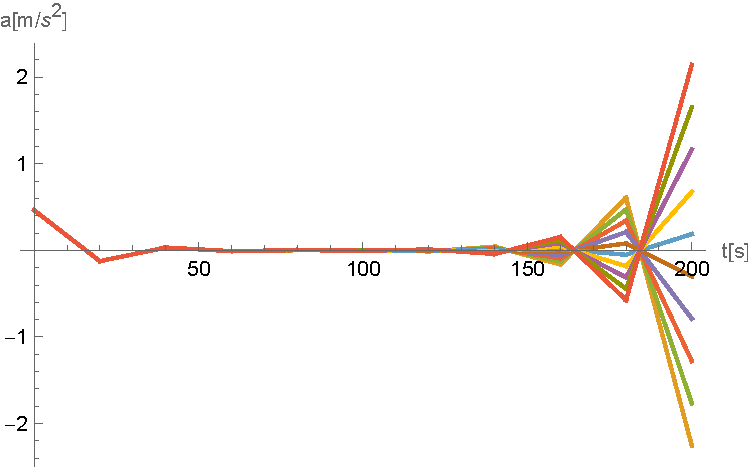
\includegraphics[width=0.7 \textwidth]{1.nal_slike/pospešek_periodično_zvezno.pdf}
    \caption{Družina funkcij poteka hitrosti in pospeška pri rešitvi za 10 semaforjev na razdaljah $L=300$ m in intervalih $t_0 = 20$ s ter začetne hitrosti $v_0 = 90$ km/h in začetnega pospeška na intervalu [-1,732 048 5, -1,732 053 0] s korakom po $0,5\, 10^{-6}$ ob upoštevanju enake hitrosti in pospeška ob prehodu semaforja.}
    \label{fig:periodično_zvezno}
\end{figure}

\section*{Opomba}

Izračuni so izvedeni pretežno v programu Wolfram Mathematica, edinole za poglavje \ref{sec:1} je uporabljen Python. Zaradi bolj realne predstavitve hitrosti, pospeškov, razdalj in intervalov semaforja so uporabljene enote z dimenzijami.